\documentclass[12pt,a4paper]{article}
\usepackage[latin1]{inputenc}
\usepackage{amsmath}
\usepackage{amsfonts}
\usepackage{amssymb}
\usepackage{graphicx}
%\usepackage[width=17.00cm, height=24.00cm, left=3.00cm, right=3.00cm, top=3.00cm, bottom=3.00cm]{geometry}
\usepackage[top=3cm,bottom=3cm,left=3cm,right=3cm,headsep=10pt,letterpaper]{geometry} % Page margins
\author{Zhen-Xiong Yuan}
\begin{document}
\title{Two Step SAR ADC} \maketitle
Successive-approximation-register (SAR) analog-to-digital converter (ADC) have been widely used due to its lower power consumption, inherent analog simplicity and compatibility to technology scaling. However, the conversion resolution ($\sim$ 8-10 bits) and speed of SAR ADC is still largely limited by mismatches between elements and its serial decision process. A few works have been reported to combine the pipeline architecture with SAR in an attempt to achieve higher resolution as well as higher conversion speed. 

A typical pipelined SAR ADC is shown in figure. , in which two SAR ADC are employed in the first and the second conversion stages connected by a residue amplifier (RA) to enable pipeline. Compared to a conventional pipelined ADC, a SAR typically offers a higher resolution in the first stage due to its simple analog structure. As a result, the front-end matching accuracy as well as the precision specs for the RA are both much relaxed. In addition, since SAR ADC typically utilizes a switched-capacitor DAC to produce the successive decision thresholds during bit cycles, so there is no necessary to introduce additional multiplying DAC (MDAC) as in conventional pipelined ADC.

This article is organized as follows. Section~\ref{sec:error} describes the prototype ADC architecture and analysis of the static error source in the two-step ADC. Section~\ref{sec:off} introduces the off-line calibration methods. Section~\ref{sec:back} describes some of background calibration methods. 

\section{Static Error Analysis}\label{sec:error}
Figure shows the block diagram of the prototype 12 bit two-step SAR ADC. In this work, we use the 6+8 bit two-step structure with 1 bit inter-stage redundancy. Since the two SAR ADC employ the MCS structure, basically the LSB of the first ADC is the same as the MSB of the second one.  Therefore, this structure will give a 12 bit resolution ADC in total.

In the 180 nm process we used to implement the prototype, the inter-stage redundancy can tolerate at most 50 mV non-ideal errors with a 1.8 V reference for both sub-ADC. The nominal inter-stage gain between the two stages is chosen to be $16\times$ (instead of $32\times$) to decease te output swing of the residue amplifier, thereby reducing its distortion and providing the 1 bit inter-stage redundancy.

For every input voltage, a single conversion will give us a 6 bit digital output $D_{FE}$ from the first stage, and a 8 bit digital output $D_{BE}$ from the second stage. From these two digital words, we can extract the 12 bit final digital output. In a ideal case, the final output code and LSB of the 12 bit ADC is given below:
\begin{gather}
	D_{OUT} = \left\lfloor \dfrac{D_{FE}}{2} \right\rfloor \times 128  + D_{BE} \\
	LSB = \dfrac{LSB_{BE}}{16}
\end{gather}
where $LSB_{BE}$ is the LSB of the second ADC. However, there are many kinds of static errors which will in turn make a violation to the ideal case. We list some of the static errors below:
\begin{enumerate}
	\item Non-linearity of the first ADC
	\item Offset of the comparator of the first ADC
	\item Gain error of residue amplifier
	\item Offset of the residue amplifier
	\item Offset of the comparator of the second ADC
	\item Gain error of the first ADC
	\item Gain error of the second ADC
	\item Non-linearity of the gain of the residue amplifier
	\item Non-linearity of the second ADC
\end{enumerate}

We will analysis some of the static error in detail. In order to demonstrate the effects of the error sources, we take a 4-bit first stage MCS-SAR ADC for example, and plot the amplified residue voltage.

\subsection{Gain error of the residue amplifier}
Figure.~\ref{fig:gain_error} shows the effect of residue amplifier's gain error on the output of the first ADC and on the input voltage of the second SAR ADC.
\begin{figure}[!h]
	\centering
	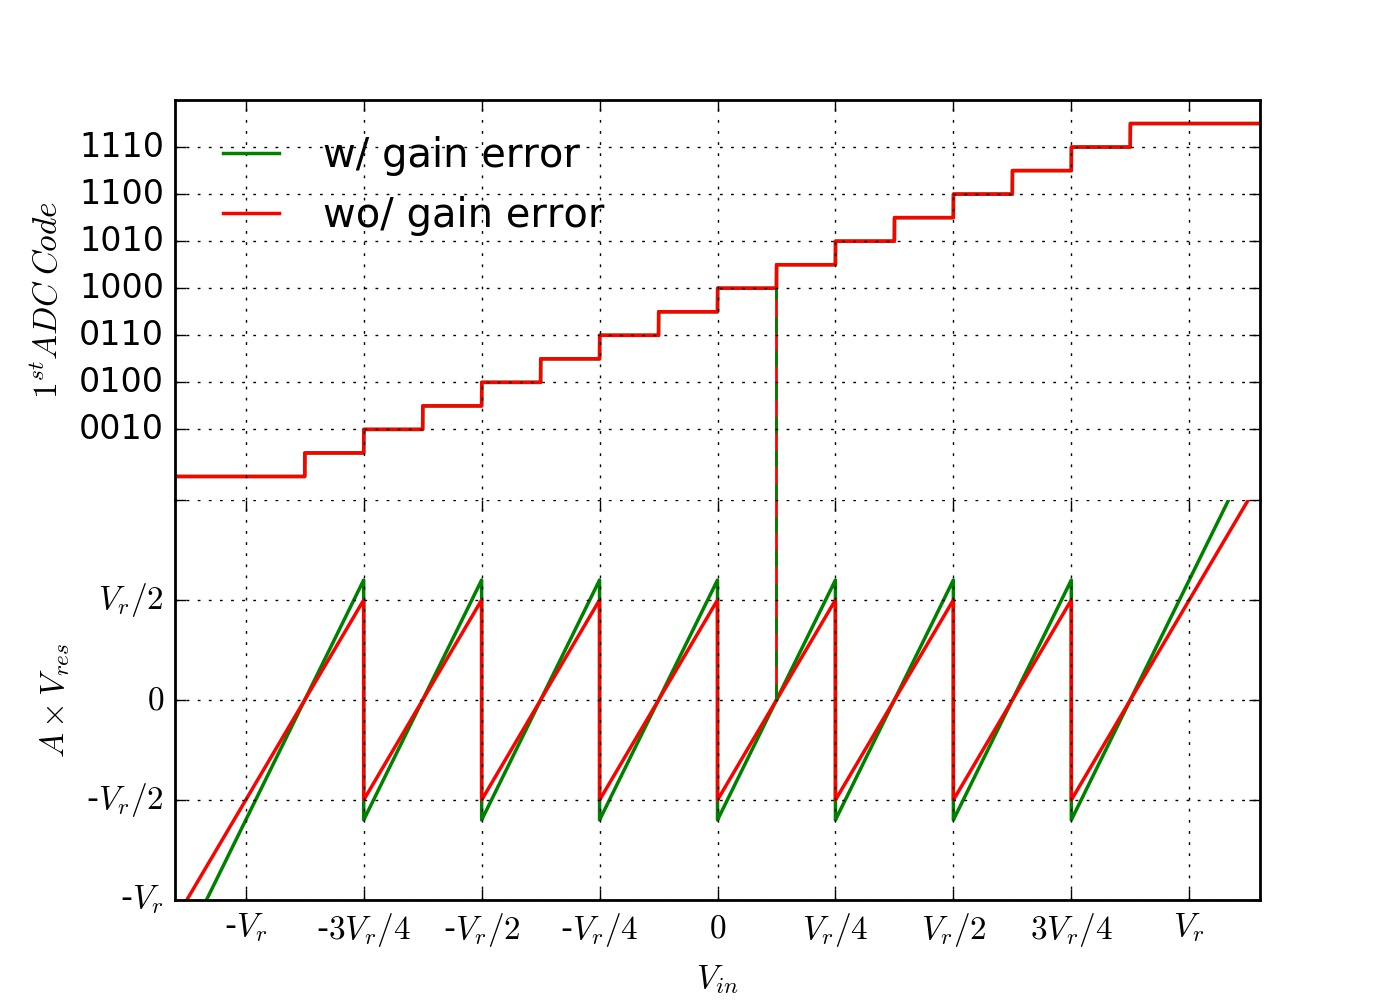
\includegraphics[width=0.85\textwidth]{figures/gain_error.jpg}
	\caption{Gain error of the amplifier on the $D_{FE}$ and the amplified residue voltage}
	\label{fig:gain_error}
\end{figure}

\subsection{Non-linearity of the first ADC}
Figure.~\ref{fig:adc_error} shows the effect of non-linearity of the first ADC on the output of the first ADC and on the input voltage of the second SAR ADC.
\begin{figure}[!h]
	\centering
	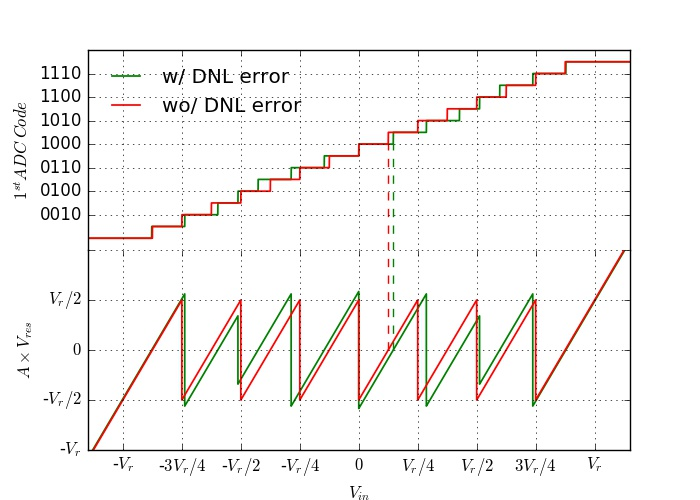
\includegraphics[width=0.85\textwidth]{figures/ADC1_dnl.jpg}
	\caption{Non-linearity of the first ADC on the $D_{FE}$ and the amplified residue voltage}
	\label{fig:adc_error}
\end{figure}

\section{Off-line Calibration with Ramp Test Signals} \label{sec:off}

\section{Background Calibration Methods}\label{sec:back}


\end{document}